\documentclass[10pt,twocolumn,letterpaper]{article}

\usepackage[review]{cvpr}      % To produce the REVIEW version

\usepackage{booktabs}
\usepackage{amssymb}
\usepackage{amsmath,amsfonts}
\usepackage{array}
\usepackage{tabularx}

\definecolor{cvprblue}{rgb}{0.21,0.49,0.74}
\usepackage[pagebackref,breaklinks,colorlinks,allcolors=cvprblue]{hyperref}

\def\confName{CVPR}
\def\confYear{2027}

%%%%%%%%% TITLE - PLEASE UPDATE
\title{Learning from Filter-Corrected Labels: Supplementary Material}

%%%%%%%%% AUTHORS - PLEASE UPDATE
\author{
    Anonymous Submission
}


\begin{document}
\maketitle

\appendix

\section{Interpretation of the Pairwise Risk}
The main text uses an unnormalized one-versus-rest risk. For a fixed distribution $Q$, let $q_i(x)=Q(y=i\mid x)$ and $\pi_i=Q(y=i)\in(0,1)$. For independent draws and the tie-aware indicator loss, the risk $U_i$ has the identity
\begin{equation}
U_i(f)=2\pi_i(1-\pi_i)[1-\mathrm{AUC}_{Q,i}(f)].
\end{equation}
To verify it, condition the first weighted loss on one positive and one negative example. The posterior factors yield $\pi_i(1-\pi_i)$ times the conditional ranking error, which equals $1-\mathrm{AUC}_{Q,i}$. Exchanging the independent examples gives the same value for the reverse term. Adding the two terms proves the identity, including ties. On the uncorrected subset, $Q=P(x,y\mid s=1)$ and its class priors must be used. This identity concerns exact posteriors and an indicator risk. It supplies no consistency or convergence guarantee for the practical mixed-posterior logistic objective.

% VERIFY V2: recover split files and complete Caltech/EuroSAT validation and test counts.
\section{Details of Datasets}
We use five image-classification benchmarks that cover natural images,
fine-grained recognition, and remote sensing. All image
inputs are converted to RGB and resized to $224\times224$ before CLIP
encoding. The encoder is frozen after feature extraction. Training-set sizes
follow the main paper and are specified below for each dataset. The reported
test set is never used for model selection.

\begin{itemize}
    \item \textbf{CIFAR-100 \cite{krizhevsky2009cifar100}.} This dataset
    contains 60,000 $32\times32$ color images from 100 classes. We use the
    official 50,000-image training split, divide it into 45,000 training and
    5,000 validation images, and evaluate on the official 10,000-image test
    split.

    \item \textbf{Tiny-ImageNet \cite{le2015tinyimagenet}.} This benchmark
    contains 200 classes, with 500 training images and 50 validation images per
    class at $64\times64$ resolution. We divide the 100,000 training images
    into 90,000 training and 10,000 validation images. The official labeled
    validation split is used as the test set because the challenge test labels
    are not publicly available.

    \item \textbf{Caltech-101 \cite{fei2004caltech101}.} The dataset contains
    101 object classes and a ``BACKGROUND\_Google'' category. Our experimental
    label space includes the background category, giving 102 classes, with
    2,945 images used for training as reported in the main paper.
    

    \item \textbf{Food-101 \cite{bossard2014food101}.} Food-101 contains
    101 food categories and 101,000 images. Its official split has 75,750
    training images and 25,250 test images. Using seed 42, we randomly
    reserve 100 images per class from the official training split for
    validation, leaving 650 images per class for training. This yields
    65,650 training and 10,100 validation images. We evaluate on the
    unchanged official test split of 25,250 images.

    \item \textbf{EuroSAT \cite{helber2018eurosat}.} This remote-sensing
    benchmark contains 27,000 RGB images from 10 land-use classes at
    $64\times64$ resolution. Our experiments use 21,600 training images,
    corresponding to 80\% of the dataset, as reported in the main paper.
\end{itemize}

CLIP generates hard pseudo-labels and supplies normalized image features, class-text embeddings, and class posteriors. To construct the FCL split, we group training images by the maximum-probability CLIP class and average their features within each group. The farthest instances are selected for simulated correction at nominal rate $\rho=0.3$. The observed-label cache stores $y_{\mathrm{obs}}$ and $s$: benchmark labels replace the selected labels when $s=0$, while the original CLIP labels are retained when $s=1$. AUC-C uses the CLIP posterior and detached classifier posterior for its pair weights.

\begin{table*}[t]
\caption{Test accuracy (\%) of the additional baselines on five datasets. Implementation details are given in Additional Baseline Comparison.
The best and second-best results within this table are shown in bold and
underlined, respectively.}
\label{tab:supp-additional-baselines}



\centering
\small
\setlength{\tabcolsep}{4pt}
\begin{tabular*}{\textwidth}{@{\extracolsep{\fill}}cccccc}
\toprule
Method & \textbf{CIFAR-100} & \textbf{Caltech-101} & \textbf{EuroSAT} & \textbf{Food-101} & \textbf{Tiny-ImageNet} \\
\midrule
CLIP-Zero-CE~\cite{radford2021clip} & 78.44 & 87.90 & 45.19 & 90.57 & 77.78 \\
Random-Filter-CE & 80.78 & 89.29 & 55.33 & 91.22 & 81.21 \\
FCL-Filter-CE & 81.94 & \underline{89.40} & 58.41 & 91.75 & 82.16 \\
Xie-Trim-AUC~\cite{xie2024wsauc} & 75.90 & 81.68 & 37.41 & 88.34 & 75.50 \\
FixMatch*~\cite{sohn2020fixmatch} & \underline{83.58} & 87.44 & \underline{90.11} & 92.01 & \underline{83.52} \\
SoftMatch*~\cite{chen2023softmatch} & 62.66 & 16.13 & 70.52 & \underline{92.04} & 82.63 \\
CLIP-Margin-CE & 78.44 & 87.90 & 45.19 & 90.54 & 77.78 \\
FCL (ours) & \textbf{85.02} & \textbf{96.20} & \textbf{93.44} & \textbf{94.78} & \textbf{84.23} \\
\bottomrule
\end{tabular*}

\end{table*}

\section{CLIP Class Descriptions}
For each class, CLIP encodes the text template \texttt{a photo of a \{class\}.}. Underscores in class names are replaced by spaces. Normalized text and image embeddings determine class scores. The maximum-probability class supplies the hard pseudo-label, while the full class distribution supplies the prior in the AUC-C weights. CLIP does not generate integer responses to instruction prompts.

\section{Number of Training Epochs and Epoch Curves}
Figure~\ref{fig:cifar-epoch} compares validation accuracy across epochs on CIFAR-100. FCL reaches higher validation accuracy than the compared baselines.

\begin{figure}[t]
\centering
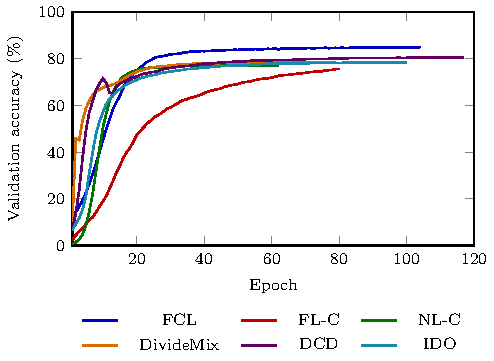
\includegraphics[width=\columnwidth]{./Figures/cifar100-epoch.pdf}
\caption{Validation accuracy by epoch on CIFAR-100. The plotted values are
read from the per-epoch validation logs.}
\label{fig:cifar-epoch}
\end{figure}

\section{Additional Baseline Comparison}
This section adds baselines using the same frozen CLIP features, data
partitions, and test protocol as the main experiments. Xie-Trim-AUC,
FixMatch and SoftMatch are cache-level adaptations; CLIP-Margin-CE is a separate margin-weighted control. Label access and
method-specific procedures are described below.

\begin{table*}[t]
\caption{Best validation accuracy (\%) on EuroSAT under different frozen
CLIP feature extractors. A star denotes a cache-level adaptation.}
\label{tab:supp-feature-extractors}



\centering
\small
\setlength{\tabcolsep}{5pt}
\begin{tabular*}{\textwidth}{@{\extracolsep{\fill}}ccccc}
\toprule
Feature extractor & \shortstack{DivideMix*~\cite{li2020dividemix}} & DCD*~\cite{mu2025dcd} & IDO*~\cite{zhang2025ido} & FCL (ours) \\
\midrule
CLIP ViT-L/14 & 44.70 & 71.78 & 43.85 & \textbf{93.44} \\
CLIP ViT-B/16 & 41.11 & 73.85 & 9.26 & \textbf{90.33} \\
CLIP ViT-B/32 & 28.44 & 73.33 & 19.48 & \textbf{88.56} \\
CLIP RN50 & 11.11 & 78.00 & 29.59 & \textbf{87.52} \\
\bottomrule
\end{tabular*}

\end{table*}

\paragraph{Compared methods.}
\begin{itemize}
    \item \textbf{CLIP-Zero-CE \cite{radford2021clip}.} This control uses CLIP's top-1 pseudo-label for
    every training image. A linear classifier is optimized with cross-entropy
    without human correction.

    \item \textbf{Random-Filter-CE.} This method corrects a uniformly random
    subset with the same size as the FCL filter area and trains on the mixed
    corrected and pseudo-label targets with cross-entropy. It isolates the
    effect of prototype-based selection.

    \item \textbf{FCL-Filter-CE.} This control uses the FCL prototype-distance
    filter and the same corrected labels as FCL, but replaces AUC-C with
    ordinary cross-entropy on the resulting mixed targets. It compares the complete training rules under a common selection mask; loss-specific attribution additionally requires matched sampling and optimization.

    \item \textbf{Xie-Trim-AUC \cite{xie2024wsauc}.} This is a cache-level adaptation inspired by
    the weakly supervised AUC formulation of Xie et al.~\cite{xie2024wsauc}.
    It keeps a fixed CLIP posterior, computes pairwise AUC losses, and trims
    high-loss instances. It does not use FCL's current-model posterior in the
    pair weights.

    \item \textbf{FixMatch* \cite{sohn2020fixmatch} and SoftMatch* \cite{chen2023softmatch}.} These controls view corrected
    instances as labeled data and uncorrected instances as unlabeled data.
    FixMatch applies a hard confidence threshold to model pseudo-labels,
    whereas SoftMatch assigns a soft confidence weight. Both are implemented
    on frozen feature caches with small feature perturbations.

    \item \textbf{CLIP-Margin-CE.} This control converts the top-two CLIP score margin into a pseudo-label weight for cross-entropy. It does not implement DeFT's learned positive/negative prompts or encoder adaptation~\cite{wei2024deft}, so its scores are not reported as a reproduction of DeFT.
\end{itemize}

Table~\ref{tab:supp-additional-baselines} reports the corresponding test
accuracies. FCL (ours) achieves the best result in every dataset among the
methods shown here. The SSL-style methods are competitive on some datasets,
while their performance varies substantially across domains. The FCL-specific controls compare selection under CE and the complete FCL training rule under prototype selection. The results favor prototype selection and FCL in these implementations; they do not establish why mixed-label CE is weaker or isolate sampler effects.

\section{Impact of Different Feature Extractors}
The filtering step depends on the geometry of the feature space, so the
backbone can affect both prototype quality and the downstream classifier. We
conduct a controlled EuroSAT study with ViT-L/14, ViT-B/16, ViT-B/32, and the
CLIP RN50 visual encoder. For each extractor, the images are encoded once, the
class-text scores and prototype filter are recomputed from that cache, and
cache-level adaptations of DivideMix~\cite{li2020dividemix},
DCD~\cite{mu2025dcd}, IDO~\cite{zhang2025ido}, and FCL are trained with the same split, filter rate,
optimizer, and early-stopping rule. The table reports the best validation
accuracy, which is the checkpoint-selection metric used throughout the paper.

FCL achieves the best validation accuracy for every extractor. DCD is the
strongest non-FCL control in each row, but FCL remains ahead by 21.66, 16.48,
15.23, and 9.52 percentage points for ViT-L/14, ViT-B/16, ViT-B/32, and RN50,
respectively. FCL consistently outperforms these three baselines across the
four frozen CLIP encoders evaluated on EuroSAT.

\paragraph{Controlled protocol.}
The extractor comparison changes only the visual backbone. We keep the text
template, class names, image preprocessing, filter rate, data partitions,
random seed, optimizer, and stopping rule fixed. Within each backbone, all
compared methods receive the same corrected labels and correction masks.
Image features are normalized
before prototype construction, and the class posterior is recomputed for each
backbone from the same prompt. This prevents differences in prompts or data
partitioning from being confounded with representation quality.

All methods train linear classifiers on frozen features without updating the
visual encoder.


\section{Selection and Objective Ablations}
\label{sec:supp-controlled-selection-objective}
We conduct additional controlled reruns to separate the correction strategy
from the objective used on uncorrected instances. Within each dataset, all
conditions use the same frozen CLIP ViT-L/14 feature cache and data partitions.
These reruns are reported separately from the historical main-table results.
The Caltech-101 records include the background category and therefore use the 102-class label space of the main text.

\paragraph{Controlled protocol.}
We train a linear classifier for 100 epochs using AdamW with weight decay
$10^{-4}$ and $\lambda=1$, $\mu=0.5$, and $\tau=0.5$.
OneCycleLR sets the effective initial learning rate to $5\times10^{-4}$,
increases it to $5\times10^{-3}$ over the first $15\%$ of the updates, and
then decreases it with cosine annealing to approximately $5\times10^{-5}$.
Both the initial and final division factors are 10. Class-balanced batches
contain 32 sampled classes with 32 instances per class on CIFAR-100 and
Food-101, and eight classes with eight instances per class on Caltech-101
and EuroSAT. We run training seeds
42, 43, and 44 without early stopping, select the first checkpoint attaining
the highest validation accuracy, and evaluate that checkpoint on the test set.

\paragraph{Selection and loss controls.}
Random-AUC corrects a uniformly sampled subset of
$\lfloor0.3N+0.5\rfloor$ training images and then applies the same
corrected-sample CE and uncorrected-sample AUC-C objective as FCL. The random
selection seed is fixed at 42 for all three training seeds. Prototype
selection instead corrects $\lceil0.3n_c\rceil$ instances within each
pseudo-labeled class, so its total query count is slightly higher.
Consequently, this comparison fixes the nominal rate rather than the exact
number of corrections; both counts are reported below.
The second control retains the exact prototype correction mask and uses CE
on corrected instances, but replaces AUC-C on uncorrected instances with
soft-label CE against the original fixed CLIP class distribution. The two
subset losses are averaged separately and added with $\lambda=1$.
For this objective comparison, each paired seed shares the observed labels,
mask, classifier initialization, optimizer settings, and actual sampling
stream. The random-selection condition has different observed labels and
is not claimed to share the same sampling stream.

\begin{table*}[t]
\caption{Test accuracy (\%) in additional controlled selection and objective
reruns. Results are mean $\pm$ sample standard deviation over training seeds
42, 43, and 44. Query counts are shown as prototype/random. The soft-CE
condition uses the same prototype mask as FCL. Caltech includes the
background category and uses the 102-class label space of the main text.}
\label{tab:supp-controlled-selection-objective}
\centering
\small
\setlength{\tabcolsep}{4pt}
\begin{tabular*}{\textwidth}{@{\extracolsep{\fill}}lrrrr}
\toprule
Dataset & \shortstack{Queries\\prototype/random} &
\shortstack{Prototype + AUC-C\\FCL} & Random + AUC-C &
\shortstack{Prototype +\\CLIP soft-CE} \\
\midrule
CIFAR-100 & 13,546/13,500 & $83.420\pm0.010$ & $83.633\pm0.032$ & $82.463\pm0.055$ \\
Caltech-101 & 914/884 & $95.688\pm0.012$ & $92.610\pm0.108$ & $96.322\pm0.104$ \\
EuroSAT & 6,485/6,480 & $92.852\pm0.037$ & $94.062\pm0.093$ & $86.901\pm0.057$ \\
Food-101 & 19,738/19,695 & $94.779\pm0.008$ & $94.672\pm0.026$ & $94.595\pm0.025$ \\
\bottomrule
\end{tabular*}
\end{table*}

Table~\ref{tab:supp-controlled-selection-objective} shows that the effect of
selection depends on the dataset. Random-AUC exceeds prototype-based FCL
by 0.213 and 1.210 percentage points on CIFAR-100 and EuroSAT, respectively.
Prototype-based FCL is higher by 3.077 points on the 102-class Caltech
protocol and by 0.107 points on Food-101. Under the same prototype mask,
AUC-C exceeds soft-label CE by 0.957, 5.951, and 0.183 points on CIFAR-100,
EuroSAT, and Food-101, respectively, whereas soft-label CE is higher by
0.635 points on Caltech-101. Thus, concentrating annotation errors in the
filtered subset does not imply a uniform downstream advantage for
prototype selection, and AUC-C does not outperform this soft-label control
on every dataset. These comparisons concern the specified rerun protocol
and do not revise the numerical results of the historical main tables.

\section{Stability across Training Seeds}
\label{sec:supp-controlled-training-seeds}
To examine training variability, we repeat the CLIP-based prototype FCL
condition with three independent training seeds under the protocol in
Section~\ref{sec:supp-controlled-selection-objective}. The feature cache,
data partitions, CLIP labels, and prototype correction mask are held fixed;
the seeds change the classifier initialization and sampling randomness.
The test set is evaluated after validation-based checkpoint selection in
each run. Table~\ref{tab:supp-controlled-training-seeds} reports every seed,
the mean and sample standard deviation, and the two-sided 95\% Student-$t$
interval for the mean. With three seeds, the interval is
$\bar a\pm4.303s/\sqrt{3}$, where $s$ uses two degrees of freedom.

\begin{table*}[t]
\caption{CLIP-based prototype FCL test accuracy (\%) under three training
seeds in the additional controlled reruns. SD is the sample standard
deviation. The 95\% interval concerns the mean over training seeds, with
data, VLM labels, and correction masks fixed. Caltech includes the
background category and uses the 102-class label space of the main text.
These values are not multi-seed estimates of the historical main-table
entries.}
\label{tab:supp-controlled-training-seeds}
\centering
\small
\setlength{\tabcolsep}{4pt}
\begin{tabular*}{\textwidth}{@{\extracolsep{\fill}}lrrrrr}
\toprule
Dataset & Seed 42 & Seed 43 & Seed 44 & Mean $\pm$ SD & 95\% CI \\
\midrule
CIFAR-100 & 83.410 & 83.420 & 83.430 & $83.420\pm0.010$ & $[83.395, 83.445]$ \\
Caltech-101 & 95.674 & 95.694 & 95.694 & $95.688\pm0.012$ & $[95.658, 95.717]$ \\
EuroSAT & 92.815 & 92.889 & 92.852 & $92.852\pm0.037$ & $[92.760, 92.944]$ \\
Food-101 & 94.776 & 94.772 & 94.788 & $94.779\pm0.008$ & $[94.758, 94.799]$ \\
\bottomrule
\end{tabular*}
\end{table*}

The sample standard deviations range from 0.008 to 0.037 percentage points
in these four reruns, indicating limited variation from initialization and
sampling under the fixed protocol. This uncertainty does not include new
data splits, VLM generations, or correction masks. Moreover, these reruns
use their own verified inputs and explicit training schedule; their seed-42
results do not coincide with all historical main-table entries. They
therefore assess repeatability under the stated conditions, rather than
supplying error bars for those earlier entries or establishing a multi-seed
ranking against the historical single-seed baselines.

\section{Filter-Corrected Qwen Labels}
\label{sec:supp-qwen-labels}
We examine whether prototype-based correction also improves labels from an instruction-following VLM. We denote corrected CLIP labels by FCL-C and corrected Qwen labels by FCL-Q; both names refer to training-label sets rather than trained classifiers. This additional study uses Qwen2.5-VL-7B-Instruct with the English class-list prompt and greedy decoding constrained to legal class identifiers. The model uses a $448\times448$-equivalent visual pixel budget. It is a separate labeling experiment, while the frozen CLIP ViT-L/14 features and verified data partitions are shared with the controlled CLIP reruns in the main paper. The Qwen model is not updated. Its generated class identifiers are discrete annotations, not calibrated class probabilities.

For each Qwen-assigned class, we average the normalized CLIP image features and select the farthest $\lceil0.3n_c\rceil$ instances, where $n_c$ is the number of images assigned to class $c$. Only selected annotations are replaced by benchmark labels. UL-ER and FL-ER measure the Qwen error rates before correction within the unselected and selected subsets, respectively. Random-M corrects the same number of uniformly sampled instances and is averaged over selection seeds 42, 43, and 44. We report CIFAR-100, Food-101, EuroSAT, and Tiny-ImageNet, which are the datasets with complete Qwen label records in this table.

\begin{table*}[t]
\caption{Qwen training-label quality (\%). The two blocks report accuracy and subset error rates before correction, followed by accuracy after prototype correction (FCL-Q) or same-count random correction (Random-M, mean $\pm$ sample standard deviation over three selection seeds). Gain is measured in percentage points (pp).}
\label{tab:supp-qwen-labels}
\centering
\small
\setlength{\tabcolsep}{4pt}
\begin{tabular*}{\textwidth}{@{\extracolsep{\fill}}lrrr}
\toprule
\multicolumn{4}{l}{\textit{(a) Before correction}} \\
\midrule
Dataset & Qwen & UL-ER & FL-ER \\
\midrule
CIFAR-100 & 47.107 & 47.118 & 66.305 \\
Food-101 & 51.484 & 39.829 & 68.720 \\
EuroSAT & 44.384 & 46.242 & 77.459 \\
Tiny-ImageNet & 28.413 & 65.437 & 85.860 \\
\midrule
\multicolumn{4}{l}{\textit{(b) After correction}} \\
\midrule
Dataset & FCL-Q & Random-M & Gain (pp) \\
\midrule
CIFAR-100 & 67.064 & $63.099\pm0.071$ & $+19.958$ \\
Food-101 & 72.148 & $66.048\pm0.145$ & $+20.664$ \\
EuroSAT & 67.644 & $61.046\pm0.026$ & $+23.259$ \\
Tiny-ImageNet & 54.267 & $49.898\pm0.056$ & $+25.853$ \\
\bottomrule
\end{tabular*}
\end{table*}

Table~\ref{tab:supp-qwen-labels} shows that the selected subsets contain more annotation errors than the unselected subsets on all four datasets. FCL-Q raises label accuracy by $19.958$--$25.853$ percentage points over the original Qwen annotations and exceeds the same-count random control in every row. Together with the CLIP comparison, these results support prototype distance as a way to concentrate a limited correction budget on erroneous labels across two VLM label sources. This conclusion concerns annotation quality; downstream classification also depends on the training objective and the residual label errors.

{
    \small
    \bibliographystyle{ieeenat_fullname}
    \bibliography{main}
}

\end{document}
